 \label{desenvolvimento_eletromecanica}

Máquina elétrica é um dispositivo capaz de transformar energia mecânica em elétrica ou vice-versa. Quando a máquina converte energia elétrica em energia mecânica ela trabalha como um motor e quando transforma energia mecânica em elétrica ela trabalha como um gerador, sendo assim, toda máquina elétrica pode funcionar dos dois jeitos, tanto como gerador como motor. \cite{chapman}  \\

No projeto em questão, será usado motores de indução trifásicos com o intuito de acionar um sistema com objetos desbalanceados presos em uma bancada, gerando assim uma vibração nesta bancada. Para realizar esta vibração, a velocidade do motor será alterada com o uso de um inversor de frequência. O conjunto motor+inversor dimensionado deverá atender o torque solicitado e as velocidades solicitadas por todo o sistema.\\
\\
\textbf{MOTOR DE INDUÇÃO TRIFÁSICO}\\

Os motores de indução trifásicos ou monofásicos são os mais amplamente usados em acionamentos elétricos, pois sua eficiência é alta, em torno de 85\%.\cite{WEG}
\\

\textbf{Princípio de funcionamento do motor de indução}: quando se aplica uma tensão trifásica no estator, gera-se um conjunto de correntes trifásicas circulando no estator. Um campo magnético girante então é produzido e este campo passa pelas barras do rotor e induz tensão nelas. Como existem dois campos magnéticos, um no estator e um no rotor, aparecerá uma força entre o rotor e o estator que fará com que o rotor gire, pois este está solto e seu eixo montado em rolamentos, gerando assim torque no seu eixo \cite{chapman}. A velocidade de rotação do campo magnético é dada por:


    \begin{equation}\label{Rotação de Campo Mag.}
            Nsinc=(120*f)/P
    \end{equation}

onde f é a frequência do sistema de alimentação em hertz e P é o número de polos da máquina. \cite{chapman}
\\

O rotor não gira na velocidade síncrona, pois se isso acontecesse o rotor estaria estacionário em relação ao campo magnético, logo, não haveria tensão induzida e consequentemente não haveria corrente nem campo magnético no rotor. Sem campo magnético no rotor o torque induzido seria zero e o motor perderia velocidade por causa do atrito. Portanto, um MIT pode ganhar velocidade até próximo da velocidade síncrona, mas nunca alcança-la exatamente.\cite{chapman}
\\

A diferença entre a velocidade síncrona e a velocidade do rotor, chama-se velocidade de escorregamento (Nesc). \cite{chapman}

    \begin{equation}\label{Velocidade de Escorregamento .}
            Nesc=Nsinc-Nm
    \end{equation}


Segundo \cite{chapman} outro termo usado, é o chamado escorregamento (S), que é a velocidade relativa expressa em uma base por porcentagem.


  \begin{equation}\label{Escorregamento S}
           S=(Nesc/Nsinc) x 100\%
    \end{equation}

A velocidade mecânica do rotor pode ser expressa em função do escorregamento e da velocidade síncrona, logo:


  \begin{equation}\label{Velocidade Mecânica do Rotor}
         Nm=(1-S)Nsinc
    \end{equation}

O tipo de máquina de indução polifásica mais comumente usada é o rotor de gaiola de esquilo como pode-se ver na figura \ref{fig:motor}, no qual barras condutoras encaixadas em ranhuras no ferro do rotor e curto-circuitadas em cada lado por anéis condutores caracterizam seu enrolamento. \cite{Fitzgerald}
\\
\begin{figure}[t]
\centering
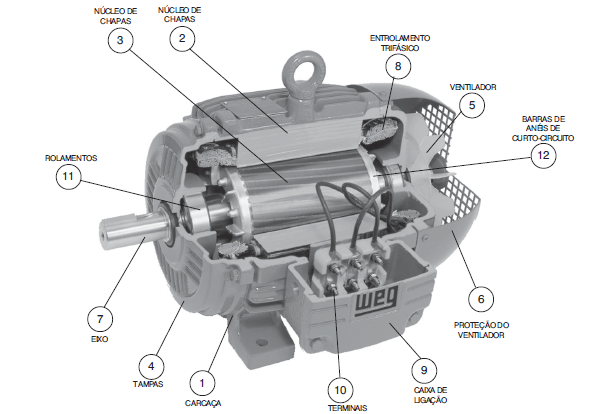
\includegraphics[keepaspectratio=true,scale=0.8]{figuras/motor.png}
\caption{Motor gaiola de esquilo. Fonte:\cite{WEG}}
\label{fig:motor}

\end{figure}

\textbf{CURVAS CARACTERÍSTICAS DO MOTOR DE INDUÇÃO}\\

A curva de torque x velocidade mostra a relação entre o torque desenvolvido pelo motor e sua rotação. Na partida o torque será de aproximadamente 2 a 2,5 vezes o torque nominal. De acordo com o aumento da velocidade este vai diminuindo até atingir valores de 1,5 a 1,7 do torque nominal.\cite{WEG} A medida que essa velocidade aumenta o torque vai aumentando novamente até atingir seu valor de pico máximo e depois vai diminuindo até chegar no seu
valor nominal, como mostra a figura \ref{fig:curvas_motor}.
% valor nominal, como mostra a figura abaixo:

\begin{figure}[h!]
\centering
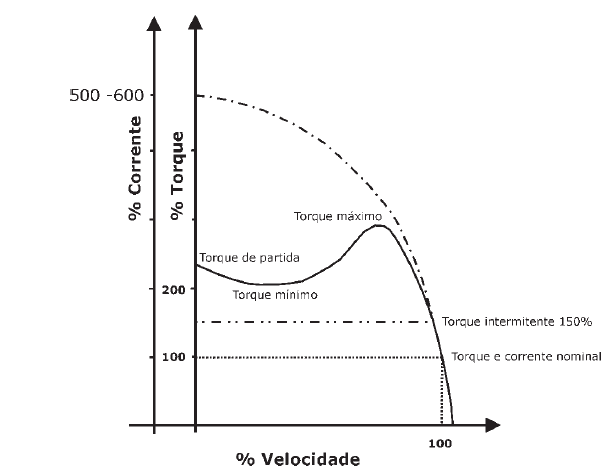
\includegraphics[scale=0.8]{figuras/grafico_motor.png}
\caption{Curvas Torque x Velocidade e Corrente x Velocidade para MI de rotor gaiola de esquilo. Fonte:\cite{WEG}}
\label{fig:curvas_motor}
\end{figure}

A curva de Corrente x Velocidade mostra a relação entre a corrente consumida pelo motor em função da velocidade. Como pode-se observar na Figura \ref{fig:curvas_motor}, quando o motor é acionado tem-se um pico de corrente de 5 a 6 vezes maior que a corrente nominal, diminuindo à medida que a velocidade aumenta até atingir um valor permanente de funcionamento.\\

\text Esses picos de corrente causado pelo acionamento de motores não é bom para a rede elétrica e para os demais aparelhos, por isso, existe maneiras de partidas mais suaves como a partida estrela-triângulo (tem o valor da corrente diminuído cerca de 1/3 da corrente de partida) e a soft-starter que é com o uso de um inversor de frequência como será explicado logo a frente.\\

\textbf{ESPECIFICAÇÕES DO MOTOR E ANÁLISE DO MOTOR}

O Motor Trifásico IP55 pode ser aplicado em bombas, ventiladores, exaustores, britadores, moinhos, talhas, compressores e outras aplicações que requeiram motores assíncronos de indução trifásicos. Pode ser utilizado, ainda, com inversores em tensões menores que 575V. \cite{WEG_catalogo}

O Motor Trifásico IP55 pode ser aplicado em bombas, ventiladores, exaustores, britadores, moinhos, talhas, compressores e outras aplicações que requeiram motores assíncronos de indução trifásicos. Pode ser utilizado, ainda, com inversores em tensões menores que 575V. \cite{WEG_catalogo}

Se ligarmos os três sistemas monofásicos entre si, como indicam as figuras \ref{fig:TRIANGULO} e \ref{fig:ESTRELA}, podemos eliminar três fios, deixando apenas um em cada ponto de ligação, e o sistema trifásico ficará reduzido a três fios L1, L2 e L3.Tensão de linha ( U ) É a tensão nominal do sistema trifásico aplicada entre dois quaisquer dos
três fios L1, L2 e L3.

\begin{figure}[!ht]
\centering
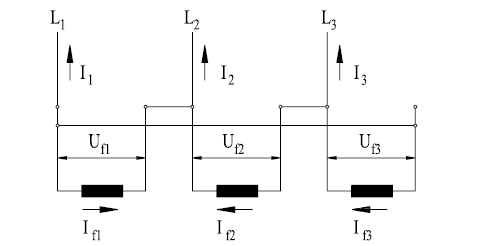
\includegraphics[scale=0.8]{figuras/TRIANGULO.png}
\caption{Ligação em Delta (triângulo). Fonte:\cite{WEG_catalogo}}
\label{fig:TRIANGULO}
\end{figure}

Ligando um dos fios de cada sistema monofásico a um ponto comum aos três, os três fios restantes formam um sistema trifásico em estrela, como pode-se ver na figura  \ref{fig:ESTRELA}. Às vezes, o sistema trifásico em estrela é “a quatro fios” ou “com neutro”. O quarto fio é ligado ao ponto comum às três fases. A tensão de linha ou tensão nominal do sistema trifásico e a corrente de linha, são definidas do mesmo modo que na ligação triângulo.\cite{WEG_catalogo}

De acordo com o abordado acima, a ligação do motor será em estrela, dado que a disponibilidade de tensão é 220V na rede elétrica local.

\begin{figure}[h!]
\centering
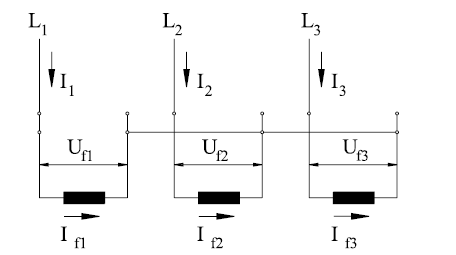
\includegraphics[scale=0.8]{figuras/ESTRELA.png}
\caption{Ligação em estrela. Fonte:\cite{WEG_catalogo}}
\label{fig:ESTRELA}
\end{figure}

Conforme as suas características de conjugado em relação à velocidade e corrente de partida, os motores de indução trifásicos com rotor de gaiola, são classificados em categorias, cada uma adequada a um tipo de carga. Estas categorias são definidas em norma (NBR 7094), e são as seguintes: N, H e D.\cite{WEG_catalogo}

Para o tipo de motor avaliado temos que a categoria de conjugado é do tipo N. \cite{WEG_catalogo}

\textbf{Categoria N:} Conjugado de partida normal, corrente de partida normal; baixo escorregamento.\cite{WEG_catalogo}

Na figura \ref{fig:conjugado_N} verifica-se como se comportam as três principais categorias de motores de indução de gaiola em função da velocidade.

\begin{figure}[H]
\centering
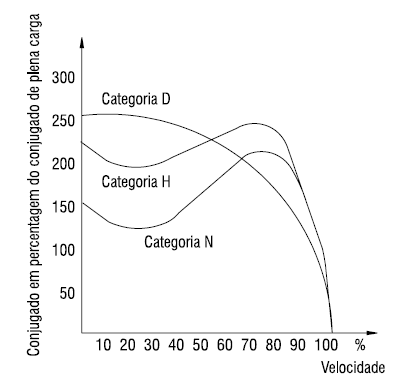
\includegraphics[scale=0.8]{figuras/conjugado_N.png}
\caption{Curvas Conjugado X Velocidade das diferentes categorias. Fonte:\cite{WEG_catalogo}}
\label{fig:conjugado_N}
\end{figure}

\begin{figure}[H]
\centering
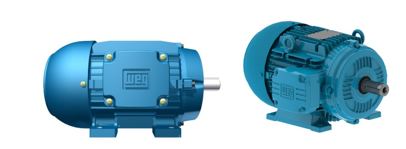
\includegraphics[scale=0.8]{figuras/motorgaiola.png}
\caption{Motor de indução trifásico do tipo gaiola. Fonte:\cite{WEG_catalogo}}
\label{fig:motorgaiola}
\end{figure}

\newpage
        \begin{table}[H]
            \begin{center}
              \begin{tabular}{|p{5cm}|p{5cm}|}
                \hline
                \textbf{Dados elétrico do motor} &
                \\ \hline
                Carcaça & 71
                \\ \hline
                Potência & 0,5HP
                \\ \hline
                Frequencia & 60Hz
                \\ \hline
                Polos & 4
                \\ \hline
                Rotação Nominal & 1720 RPM
                \\ \hline
                Escorregamento & 4,44
                \\ \hline
                Tensão Nominal & 220/380 V
                \\ \hline
                Corrente Nominal & 2.07/1.20 A
                \\ \hline
                Corrente de Partida & 10.45/5.99 A
                \\ \hline
                LP/LN & 5.0
                \\ \hline
                Corrente a vazio & 1.50/0.868 A
                \\ \hline
                Conjugado Nominal & 2.06 Nm
                \\ \hline
                Conjugado de partida & 240
                \\ \hline
                Conjugado Máximo & 250
                \\ \hline
                Categoria & N
                \\ \hline
                Classe de isolação & B
                \\ \hline
                Elevação de temperatura & 80 K
                \\ \hline
                Tempo de rotor bloqueado & 18 s (quente)
                \\ \hline
                Fator de serviço & 1.15
                \\ \hline
                Regime de serviço & S1
                \\ \hline
                Temperatura ambiente & -20 graus Celsius - +40 graus Celsius
                \\ \hline
                Altitude & 1000 m
                \\ \hline
                Proteção & IP55
                \\ \hline
                Massa aproximada & 10 Kg
                \\ \hline
                Momento de inércia & 0,00082 Kg
                \\ \hline
                Nível de ruído & 47 dB(A)
                \\ \hline
              \end{tabular}
              \caption[Informações detalhadas sobre o motor]{Informações detalhadas sobre o motor
              \protect Fonte:\cite{WEG_catalogo} }
            \label{tabela_info_motor}
        \end{center}
    \end{table}
\newpage

\begin{figure}[H]
\centering
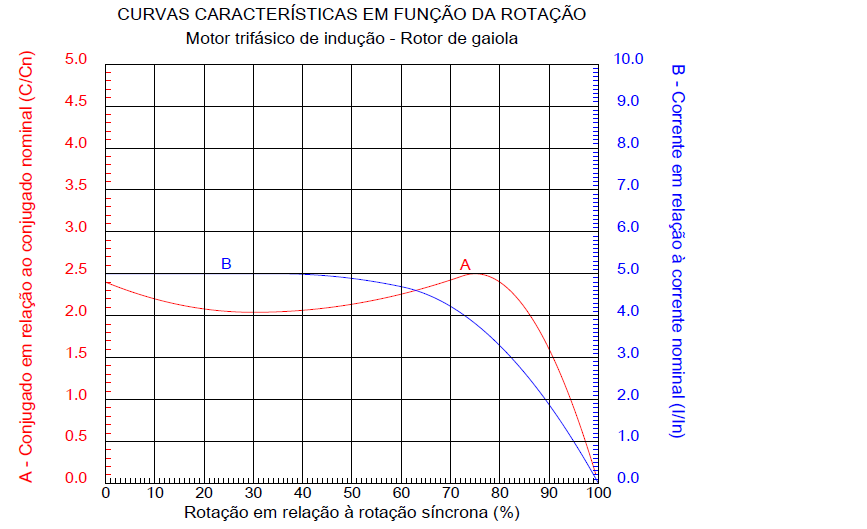
\includegraphics[scale=0.8]{figuras/motor_rota__o.png}
\caption{Curvas características em função da rotação Fonte: \cite{WEG_catalogo} }
\label{fig:motor_rota__o}
\end{figure}

\begin{figure}[H]
\centering
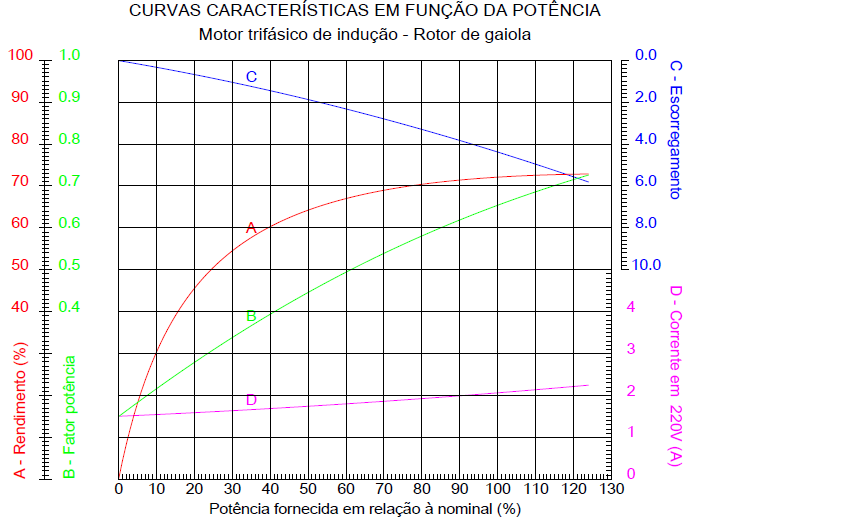
\includegraphics[scale=0.8]{figuras/Motor_potencia.png}
\caption{Curvas características em função da potência Fonte: \cite{WEG_catalogo} }
\label{fig:Motor_potencia}
\end{figure}


Como já mencionado algumas vezes neste trabalho, uma das principais preocupações que devemos ter em relação aos motores elétricos é sua temperatura de operação, cada motor possui um tipo de classe de isolamento que nada mais é que um tipo diferente de isolante em seus enrolamentos (ou a quantidade dele), esses isolantes servem, como o próprio nome diz, para isolar os fios um dos outros das bobinas, no caso dos motores gaiola, da bobina do estator.\cite{WEG_catalogo}

\begin{table}[H]
\centering
\caption{Classe de isolamento. Fonte:\cite{WEG_catalogo}}
\label{isolamento}
\begin{tabular}{|l|c|c|c|c|c|}
\hline
\multicolumn{1}{|r|}{\multirow{2}{*}{\textbf{Temperatura}}} & \multicolumn{5}{c|}{\textbf{Classe de isolamento}}             \\ \cline{2-6}
\multicolumn{1}{|r|}{}                                      & \textbf{A} & \textbf{E} & \textbf{B} & \textbf{F} & \textbf{H} \\ \hline
TA($^{\circ}$C)                                                      & 40         & 40         & 40         & 40         & 40         \\ \hline
$\alpha$ t($^{\circ}$C)                                              & 60         & 75         & 80         & 105        & 125        \\ \hline
$\Delta$ T($^{\circ}$C)                                              & 5          & 5          & 10         & 10         & 15         \\ \hline
Total ($^{\circ}$C)                                                  & 105        & 120        & 130        & 155        & 180        \\ \hline
\end{tabular}
\end{table}

\vfill
\pagebreak

\textbf{INVERSORES DE FREQUÊNCIA}\\

A tensão de rede de frequência constante é transformada em uma tensão com frequência e amplitude variáveis pelo inversor,     assim ocorre uma variação na velocidade do campo girante. O inversor de frequência é vantajoso para as indústrias, porque o controle é à distância (comunicação serial), há redução de custos (corrente de partida limitada), produtividade aumentada (velocidade de operação devidamente adequada ao processo), eficiência energética (rendimento superior a 97\%) e agilidade para os sistemas de posicionamento (partidas e frenagens acontecem em milésimos de segundos) \cite{WEG2}.
    Analisando as equações:

    \begin{equation}\label{Rotação Sinc.}
            Nsinc=(120*f)/P
    \end{equation}
    e
    \begin{equation}\label{Rotação Sinc.}
     Nm=(1-S)Nsinc
    \end{equation}

     verifica-se que a variação do escorregamento é capaz de modificar a velocidade de rotação de um motor de indução trifásico; o número de polos do motor ou da frequência da tensão no estator também modificam essa velocidade. O método mais eficaz para a variação da velocidade de rotação de motor de indução tem sido a utilização de inversor de frequência. \cite{WEG2}.

     \textbf PARTIDA E FRENAGEM DE MIT (MOTOR DE INDUÇÃO TRIFÁSICO) COM INVERSOR DE FREQUÊNCIA\\

     O inversor de frequência trabalha com rampas para partida e frenagem. Na partida é utilizada a rampa de aceleração, a velocidade inicia em zero e atinge a velocidade desejada, podendo ajudar o tempo numa faixa de milésimos de segundo.
    A frequência do rotor é maior do que a frequência do estator durante a frenagem, dessa forma é provocado um fluxo reverso da energia do rotor diretamente ao estator \cite{covino}. A rampa de desaceleração é responsável por controlar a frenagem, esse processo se dá pela redução de forma controlada da frequência aplicada ao motor.
    A figura abaixo evidencia as rampas de aceleração e desaceleração:\\

 \begin{figure}[h]
    \centering
    \label{oldr}
    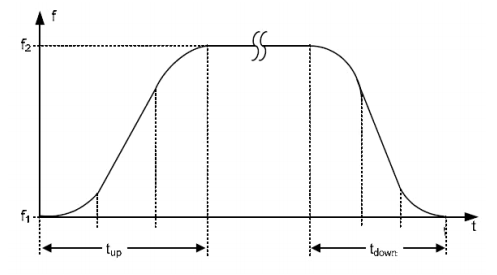
\includegraphics[keepaspectratio=true,scale=0.75]{figuras/rampa_aceleracao.png}
    \caption{Rampas de aceleração e desaceleração geradas pelo inversor de frequência \cite{siemens}.}
    \end{figure}


        O projeto contará especificamente com o inversor Power Flex 40 de 0,5CV a 380V da consagrada marca Allen Bradley, com vasta tradição de aplicabilidade na indústria.


\begin{figure}[H]
  \centering
  \label{inversor_final}
  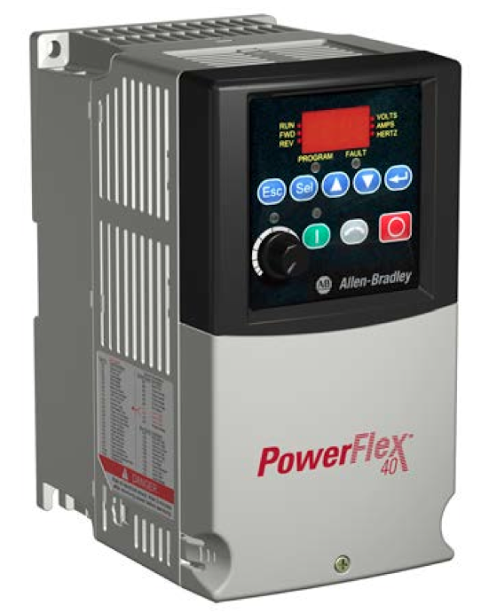
\includegraphics[keepaspectratio=true,scale=0.4]{figuras/inversor_final.png}
  \caption{Inversor Allen Bradley - Power Flex 40 \cite{allen}.}
\end{figure}

        O modelo selecionado, entrega a possibilidade de controle externo digital por suas portas analógicas e digitais. Os estudos preliminares acerca do projeto indicou uma maior número de vantagens em se utilizar o controle analógico, em razão, principalmente, de uma melhor precisão de resposta.

        O formato de controle fica baseado na entrega de grandezas elétricas como tensão e corrente por meio dos dispositivos externos que são lidos e interpretados como respostas diretas nos parâmetros.


\textbf APLICABILIDADE AO SISTEMA DA MESA DE VIBRAÇÃO\\

O inversor assume papel vital, pois uma vez que é responsável por interfacear o mecanismo de potência e controle para com a aplicação desejada, no projeto será quem, de fato, condicionará o motor a operar segundo as especificações retornadas do sistema de controle. As rotinas de testes da bancada entregam ao inversor de forma instantânea os dados de frequência de operação, e consequentemente de velocidade a qual a mesa responte com a vibração esperada.

Os parâmetros de entrada do inversor são entregues segundo o consagrado protocolo de comunicação industrial MODBUS, que se trata de uma estrutura de mensagem aberta, amplamente utilizado em razão da sua simplicidade e facilidade de implementação.\\

\textbf DIMENSIONAMENTO DE CABOS\\

Dada as cargas de maior relevância do presente projeto, inversores, um par de motores e os circuitos eletrônicos do sistema, será realizado um levantamento de carga de projeto de forma a permitir com boa aproximação a obtenção dos parâmetros dos condutores de alimentação de potencia do circuito principal e dos sub-circuitos.

    O sistema motor é constituído por uma unidade de motor WEG 0,5CV 220/380V, 1720RPM os qual apresenta, segundo o fabricante, corrente nominal de 2,07A configuração estrela (380V) totalizando 0,58A por fase.

    O Inversor, Allen Breadley 0,5Cv 380V, designados para o controle de acionamento e velocidade de rotação do projeto, apresentam para tal, um autoconsumo de aproximadamente 50W, contribuindo com uma corrente de 0,13A.

    As cargas secundárias constituídas pelos sistemas de monitoramento e controle acoplados ao sistema não devem  ser menosprezadas, no entanto para fins de dimensionamento, será considerada a alimentação por uma fonte retificadora DC com entrega máxima de 2A.

    A tabela abaixo representa um compilado dos dados de corrente do projeto e os respectivos resultados dos dimensionamentos de secção mínimos segundo a normatização vigente (NBR 5410, NBR6818 e EB98 ABNT).

    \begin{table}[h]
  \centering
  \label{tab01}

  \begin{tabular}{llllll}
    \toprule
    \textbf{Item} & \textbf{Qtd} &
        \textbf{Potência} & \textbf{Corrente Tot.}  & \textbf{Corrente/f}  &
        \textbf{Secção/F NBR 6418} \\
    \midrule
    Motor & 1 & 370W & 2,07A & 0,58A & 2,5mm2 \\
    Inversor & 1 & 50W & 0,13A & 0,07 & 2,5mm2 \\
    Circ. COntrole & 1 & 24W & 2A & 2A(Fase 1) & 2,5mm2 \\
    \bottomrule
  \end{tabular}

  \caption{Correntes dos Sub-circuitos}
\end{table}

Dessa forma, levando em consideração as correntes totais por fase do sistema, chegamos aos presentes resultados para as correntes totais nos barramentos de acesso:

    \begin{table}[h]
  \centering
  \label{tab01}

  \begin{tabular}{llll}
    \toprule
    \textbf{Circuito} & \textbf{Fase 1} & \textbf{Fase 2} & \textbf{Fase 3}\\
    \midrule
    Motor e Inversor & 0,65A & 0,65A & 0,65A \\
    Controle & 2,00A & 0A & 0A \\
        Acesso de Energia & 2,65A & 0,65A & 0,65A \\
    \bottomrule
  \end{tabular}

  \caption{Correntes no Acesso de Força}
\end{table}

Dessa forma, ficando válido a bitola mínima estabelecida pela norma NBR5410 de 2,5mm para circuitos de força em todos os estágios sejam de acesso ou interconexões. \cite{NBR5410}

No que tange o dimensionamento do condutor neutro, é de boa prática que seja dimensionado segundo os mesmos parâmetros dos condutores de fase, motivado, principalmente pela carga harmônica injetada pelos circuitos não lineares dos inversores, que podem induzir a circulação de carga no condutor neutro.

    E finalmente, em relação ao condutor terra, esse deve ser capaz de atender aos requisitos mínimos de corrente de falta possivelmente possa ocorrer. Para tal, a recomendação dos fabricantes é que se utilize, no mínimo, o mesmo diâmetro dos alimentadores.

    \textbf{Polias, Correias e Transmissão de Potência}\\
    As polias são peças cilíndricas, movimentadas pela rotação do eixo do motor e pelas correias. Os tipos de polia são determinados pela forma da superfície na qual a correia se assenta.
Correias são elementos de máquinas que transmitem movimento de rotação entre dois eixos (motor e movido) por intermédio de polias. Elas são empregadas quando se pretende transmitir potência de um veio para o outro a uma distância em que o uso de engrenagens é inviável.
Para o sistema em questão será usada as polias do tipo Trapezoidal ou V múltipla. A correia em V ou trapezoidal é inteiriça, fabricada com seção transversal em forma de trapézio. É feita de borracha revestida de lona e é formada no seu interior por cordonéis vulcanizados para suportar as forças de tração.
O emprego da correia trapezoidal ou em V é preferível ao da correia plana porque:

\begin{itemize}
  \item Praticamente não apresenta deslizamento;
  \item Permite o uso de polias bem próximas;
  \item Elimina os ruídos e os choques, típicos das correias emendadas (planas). Como as correias têm características diferentes de fabricante para fabricante, é aconselhável seguir as instruções que eles forneçam.
\end{itemize}

  A partir destes elementos pretende-se selecionar a polia do tipo guia com correia do tipo trapezoidal a ser usada observando o tipo, a secção e o comprimento primitivo, potência a ser transmitida, tipos de máquina motoras e  movidas, velocidade angular da polia motora e da polia movida, distância entre os eixos da polia motora e da polia movida, distância entre os eixos das polias, na qual o comprimento máximo admitido deve ser igual a três o produto da soma dos diâmetros da polia motora e movida e finalmente o tipo de carga(uniforme, choques moderados, choques intensos).

\begin{figure}[!ht]
\centering
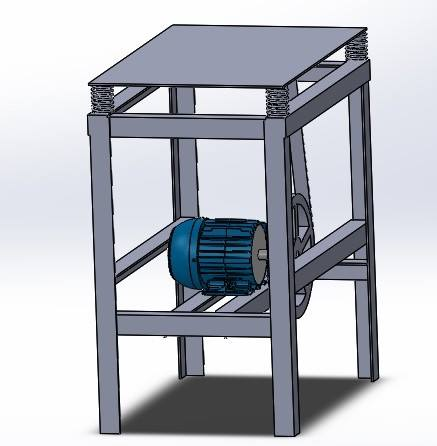
\includegraphics[scale=0.5]{figuras/motor_catia.jpg}
\caption{Esboço da base da bancada. Fonte: Autores}
\label{fig:motor_catia}
\end{figure}
